\normalfalse \difficilefalse \tdifficiletrue
\correctionfalse

%\UPSTIidClasse{11} % 11 sup, 12 spé
%\newcommand{\UPSTIidClasse}{12}

\exer{Fauteuil Roulant $\star$ \label{C2:06:54}}

\setcounter{question}{0}\UPSTIcompetence[2]{B2-13}\UPSTIcompetence[2]{C2-05}\UPSTIcompetence[2]{C2-06}
\index{Compétence C2-05}
\index{Compétence C2-06}
\index{Compétence B2-13}
\index{Fauteuil Roulant}
\ifcorrection
\else
\marginnote{\textbf{Pas de corrigé pour cet exercice.}}
\fi

\ifprof
\else
On s'intéresse au système de basculement de l'assise d'un système de fauteur roulant.
\begin{center}
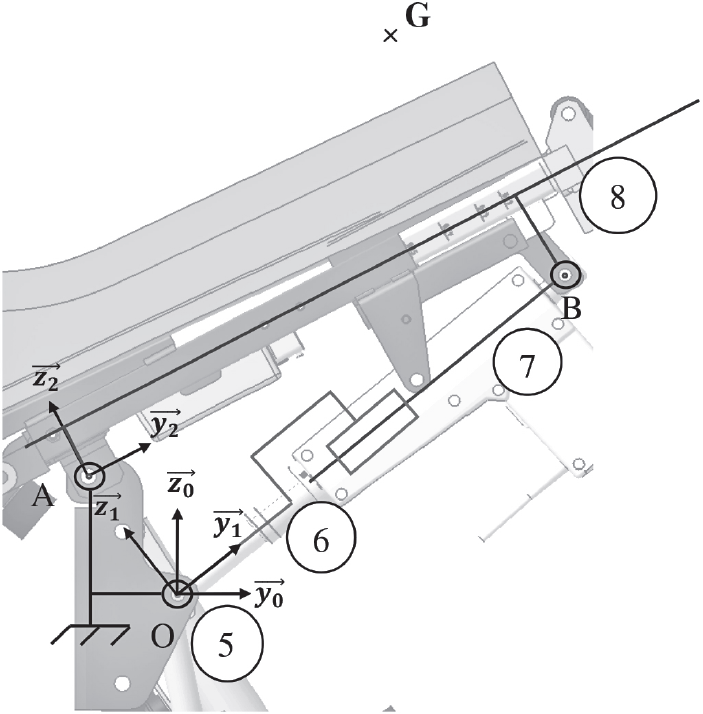
\includegraphics[width=\linewidth]{54_01}
\end{center}

\begin{center}
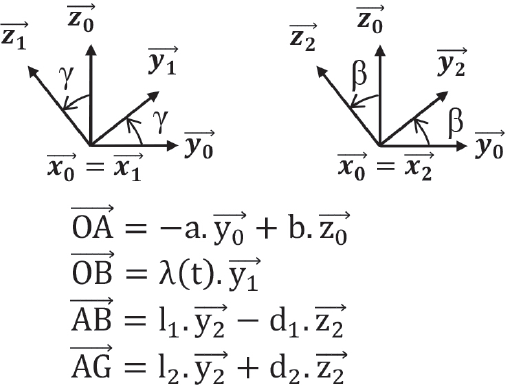
\includegraphics[width=.8\linewidth]{54_02}
\end{center}

\fi

\question{Tracer le graphe des liaisons.}
\ifprof
\else
\fi

\question{Déterminer les relations issues de la fermeture géométrique liant les paramètres $\gamma$, $\beta$ et $\lambda(t)$.}
\ifprof
\else
\fi

\question{En déduire l'expression de $\gamma$ en fonction de~$\beta$.}
\ifprof
\else
\fi

\ifprof
\else
\begin{flushright}
\footnotesize{Corrigé  voir \ref{C2:06:54}.}
\end{flushright}%
\fi